\begin{example}
    The Gamma distribution $\Gamma(p, \lambda)$ for $p, \lambda > 0$ has density
    \begin{equation*}
        f(x) = \frac{\lambda^p}{\Gamma(p)} x^{p-1} \expf{-\lambda x},
    \end{equation*}
    where $\Gamma$ is the Gamma function. Its characteristic function is $\zeta(t) = (1 - it/\lambda)^{-p}$. Hence, we can easily see that for $X_1, \ldots, X_n \simiid \Gamma(p, \lambda)$, both the sum and standardized mean of the $X_i$ follow Gamma distributions with $\sum_{i=1}^n X_i \sim \Gamma(np, \lambda)$ and $n^{-1/2} \sum_{i=1}^n X_i \sim \Gamma(np, \lambda n^{-1/2})$. The cumulant generating function of the $\Gamma(p, \lambda)$ distribution is $K(t) = p \logf{\lambda} - p\logf{\lambda - t}$, hence the cumulant of order $j$ is $\kappa_j = p\Gamma(j)\lambda^{-j}$. To be able to apply Theorem \ref{thm-edgeworth}, the condition $\zeta \in L^q(\R)$ is necessary for $q \in [1, n)$. In the case of the Gamma distribution, we have that $\zeta \in L^q(\R)$ if and only if $q > p^{-1}$, hence, Theorem \ref{thm-edgeworth} can be applied if and only if $n > p^{-1}$.

    \begin{figure}[h]
        \textbf{Simulations based on $\Gamma(1,1)$ distribution}
        \centering
        \subfloat[$n = 1$; Density and Edgeworth series \label{fig-single-gamma}]{
            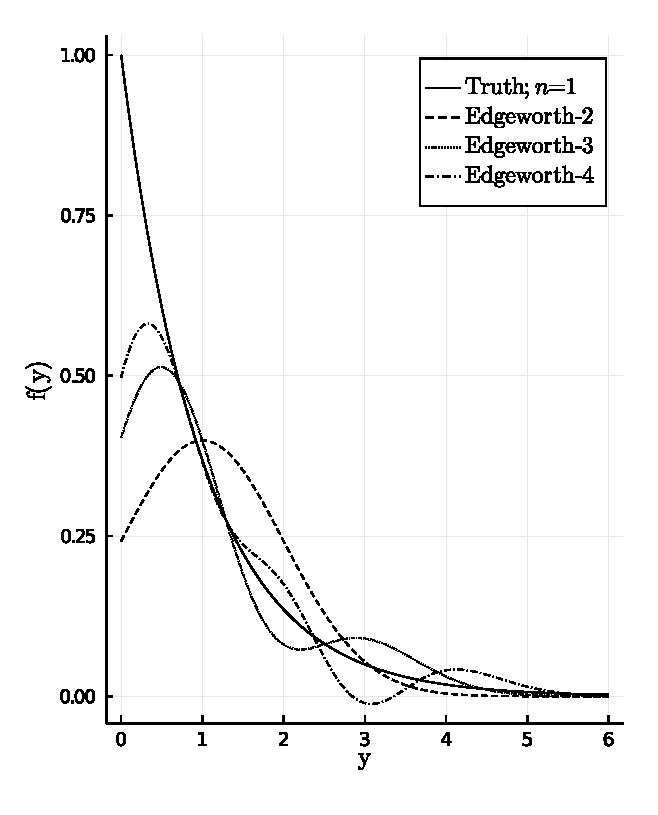
\includegraphics[width=8cm]{edgeworth_gamma11_1_terms.eps} 
        }
        \subfloat[$n = 10$; Density and Edgeworth series \label{fig-10-gamma}]{
            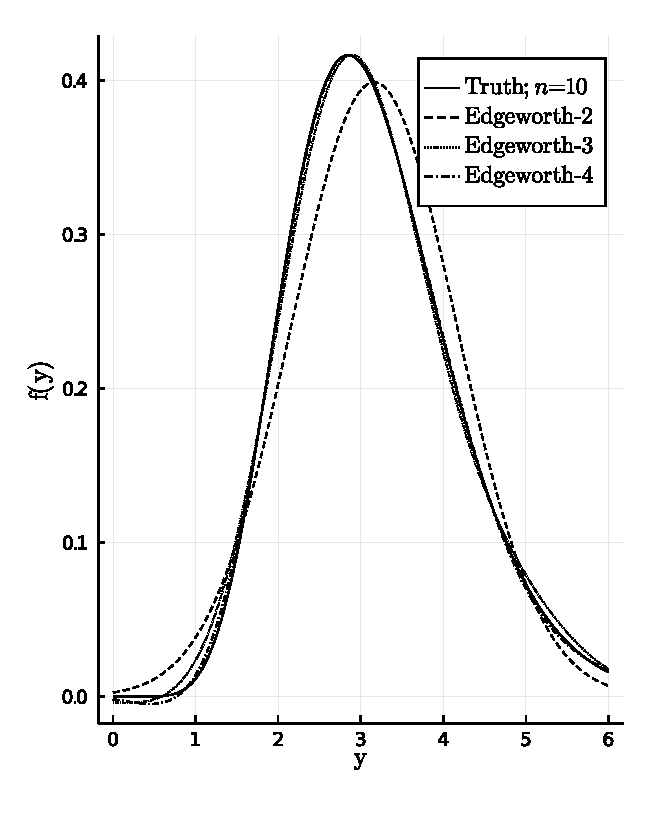
\includegraphics[width=8cm]{edgeworth_gamma11_10_terms.eps}
        }
        \qquad
        \subfloat[$n=10$; Series absolute error \label{fig-10-gamma-err-abs}]{
            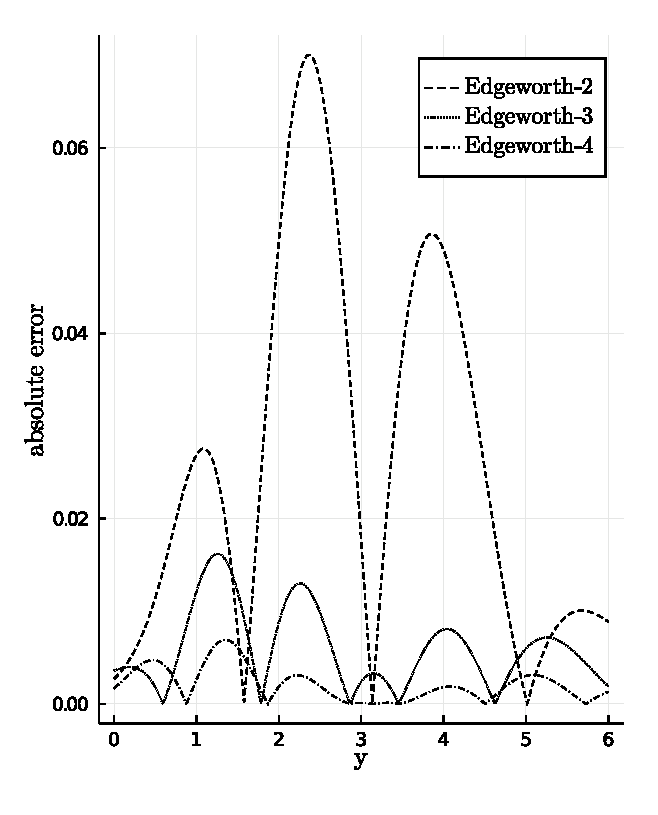
\includegraphics[width=8cm]{edgeworth_err_abs_gamma11_10_terms.eps} 
        }
        \subfloat[$n=10$; Series (log) relative error \label{fig-10-gamma-err-rel}]{
            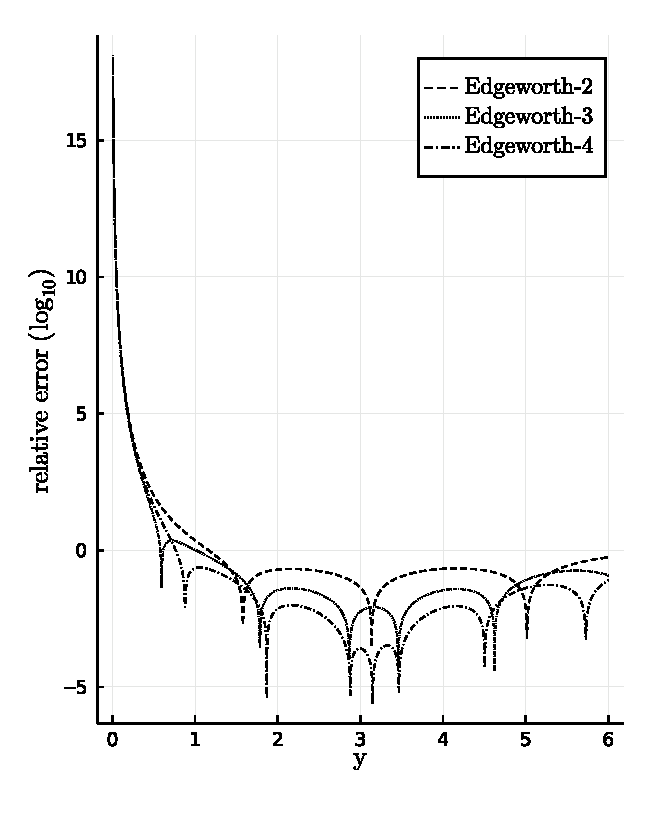
\includegraphics[width=8cm]{edgeworth_err_rel_gamma11_10_terms.eps}
        }
    \end{figure}
    
\end{example}